\documentclass[a4j]{jarticle}
\usepackage[dvipdfmx]{graphicx}
\usepackage{amsmath,ascmac}
\usepackage{bm}
\usepackage{algorithm,algorithmic}
\usepackage{listings}
\lstset{%
  language={C},
  basicstyle={\small},%
  identifierstyle={\small},%
  commentstyle={\small\itshape},%
  keywordstyle={\small\bfseries},%
  ndkeywordstyle={\small},%
  stringstyle={\small\ttfamily},
  frame={tb},
  breaklines=true,
  columns=[l]{fullflexible},%
  numbers=left,%
  xrightmargin=0zw,%
  xleftmargin=3zw,%
  numberstyle={\scriptsize},%
  stepnumber=1,
  numbersep=1zw,%
  lineskip=-0.5ex%
}
\renewcommand{\lstlistingname}{コード}
\renewcommand{\lstlistlistingname}{コード目次}

%
% 以後をレポート課題ごとに書き換える。
%

\begin{document}
\title{サンプル\LaTeX}
\author{名前（学籍番号 xxxx）}
\date{2020年 x月 y日}
\maketitle

\section{序}
\label{sec:intro}

このサンプル\LaTeX ファイルでは、\ref{sec:eqn}章では数式につい
て、\ref{sec:table}章では表について、\ref{sec:figure}章では図につい
て、\ref{sec:code}章ではソースコードの出力の仕方について、サンプル例を示した。
また、レポートの書き方の勉強には、文献\cite{Kinoshita}の一読を勧める。

% 式
\section{数式とは？}
\label{sec:eqn}

20世紀の物理学の有名な公式\eqref{eq:ein}と\eqref{eq:sch}について考える。

\begin{align}
  \label{eq:ein}
  & E = mc^2\\
  \label{eq:sch}
  & i\hbar\frac{\partial \vert\Psi\rangle}{\partial t} = H\vert\Psi\rangle
\end{align}

% 表
\section{表とは？}
\label{sec:table}

表\ref{tab:num}に集計結果を示す。

\begin{table}[ht]
  \centering
  \caption{性別集計。}
  \label{tab:num}
  \begin{tabular}[ht]{|c|c|}
    \hline
    \hline
  男性 & 10人\\
    \hline
  女性 & 10人\\
    \hline
  \end{tabular}
\end{table}

% 図
\section{図とは？}
\label{sec:figure}

図\ref{fig:tn}は貴金属の価格の推移を示す。

\begin{figure}[ht]
  \centering
  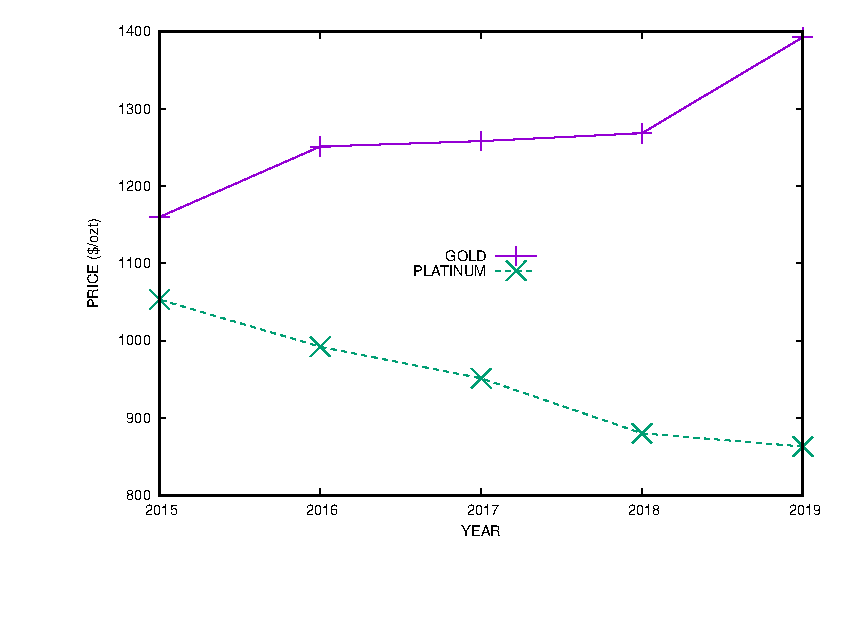
\includegraphics[width=0.8\textwidth]{sample.eps}
  \caption{金とプラチナの価格の推移。}
  \label{fig:tn}
\end{figure}

% コード
\section{コードとは？}
\label{sec:code}

コード\ref{code:sample1}とコード\ref{code:sample2}は有名なサンプルコードです。

\begin{lstlisting}[caption=ハローワールド,label=code:sample1]
  #include <stdio.h>
  int main(int argc, char **argv){
    printf("Hello world!\n"); // 有名なコード！
  }
\end{lstlisting}

\lstinputlisting[caption=ハローワールド（ファイルから読み込み）,label=code:sample2]{sample.c}

\section{まとめ}
読みやすいレポートを書きましょう。

\begin{thebibliography}{99}
\bibitem{Kinoshita} 
木下 是雄, 中公新書「理科系の作文技術」, 1981.
\end{thebibliography}
\end{document}
%%% Local Variables:
%%% mode: latex
%%% TeX-master: t
%%% End:
